\section{Reliability, Availability, Maintainability, and Safety characteristics}
\label{blRAMS}

\begin{enumerate}
	\item Reliability. Comparing with the GLAS mission, a swarm of receivers is used in this system, which is more reliable than single large telescope. Figure \ref{R} on page \pageref{R} gives a overview of subsystem contributions to satellite failures after different time span from a nonparametric analysis. More detail reliability analysis can be found in chapter risk assessment.
	\begin{figure} [H]
	\begin{center}
         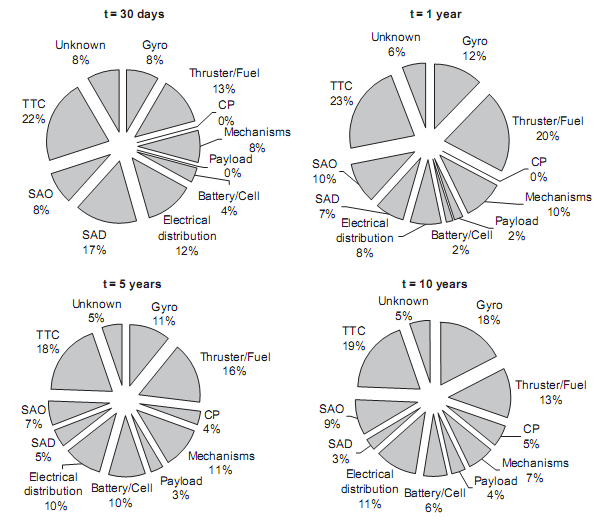
\includegraphics[width=1.0\textwidth,angle=0]{img/subsystem_reliability_analysis.png}
	\end{center}
	\caption{Subsystem contributions to satellite failures after 30 days, 1 year, 5 years, and 10years on-orbit.}
	\label{R}
	\end{figure}

	\item Availability. The system is designed functional all the time to cover the global converge. Meanwhile the laser emitter can send pulse to particular area to accomplish imperative mission. Since the system use a swarm of receivers, it is possible to switch off some of the receivers to obtain same performance(depend on exact how many receivers are used).

	\item Maintainability. Maintainability is defined as the ability of our operating system specific item to be maintained. In our case, it is not possible to do regular on-board maintenance on satellite itself, but mainly focus on ground segment. The maintenance is mainly divided into two parts, preventive maintenance and corrective maintenance. They are considering separately as follows: 
	\begin{enumerate}
		\item Preventive maintenance. During the regular system operation time, there are periodic maintenance and condition dependent maintenance.  System software or simulator servicing maintenance of ground station is mandatory and data link rate need to be adjusted for reasons sometimes. On the other hands, conditional maintenance is set to do some specific inspections to prevent something wrong in the future.
		\item Corrective maintenance. This is mainly carried out after something goes wrong. For instance, if one of the photon receiver is not functional, the system can relocate the rest of the receivers to decrease the functional influence mostly. But if the laser emitter is broken, it is no way to obtain the maintenance. Corrective maintenance is also used during analyze measurements data to obtain better resolution or accuracy.
  	\end{enumerate}

	\item Safety. The system safety is mainly considered during launch and decommission, since most of the time the satellite is on its orbit in space. The single receiver is designed small enough to avoid orbit interruption with other systems. 
\end{enumerate}
